% type de document : diaporama
\documentclass[xcolor=table]{beamer}

\usepackage[frenchb]{babel}
\usepackage[T1]{fontenc}
\usepackage[latin1]{inputenc}
\usepackage{hyperref}
\usepackage{perpage} 
\MakePerPage{footnote}
\hypersetup{
    colorlinks=true,
    linkcolor=blue,
    filecolor=magenta,      
    urlcolor=cyan,
    pdftitle={Overleaf Example},
    pdfpagemode=FullScreen,
    }
    
\usepackage{pgfplots}
\usepackage[table]{xcolor}
\usetikzlibrary{quotes}
\usepackage{graphicx}
\graphicspath{ {./images/} }
    
\setbeamercolor{titre}{bg=red,fg=white}
\setbeamercolor{texte}{bg=red!10,fg=black}
\setbeamertemplate{frametitlecontinuation}{\insertcontinuationcount}

% Choix du thème
\usetheme{JuanLesPins}

\title{Master 2 Humanit\'es num\'eriques \\
Introduction au projet encadr\'e}
\author{Gwena\"elle Patat \\
\href{mailto:gwenaelle.patat@mshb.fr}{gwenaelle.patat@mshb.fr}}
\institute{\large{Maison des Sciences de l'Homme en Bretagne}}
\date{mardi 21 septembre 2021}

\AtBeginSection[]
{
  \begin{frame}[allowframebreaks]
    \frametitle{Plan}
    \tableofcontents[currentsection, hideothersubsections]
  \end{frame}
}

\begin{document}
\frame{\titlepage}

\begin{frame}[allowframebreaks]
\frametitle{Plan}
\tableofcontents
\end{frame}

\section{Un projet de m\'ediation num\'erique de fonds d'archives}
\subsection{Partenaire}
\subsection{Th\'ematique}
\subsection{Personnes r\'ef\'erentes}
\subsection{Organisation de l'ann\'ee}
\subsection{Objectifs}

\begin{frame}[plain]
\frametitle{Un projet de m\'ediation num\'erique de fonds d'archives}
\framesubtitle{Partenaire}
\begin{itemize}
    \item Les Archives municipales de Rennes : \url{https://www.archives.rennes.fr/}
\end{itemize}
\end{frame}

\begin{frame}[plain]
\frametitle{Un projet de m\'ediation num\'erique de fonds d'archives}
\framesubtitle{Th\'ematique}
\textbf{Le sport \`a Rennes dans l'entre-deux-guerres}, en \'echo avec une exposition courant 2022 sur la cr\'eation artistique dans l'entre-deux-guerres au mus\'ee des Beaux-Arts de Rennes, et en vue des prochains jeux olympiques. R\'esonance avec la vie culturelle locale et l'actualit\'e.
\newline
\newline
Valoriser des lieux, des b\^atiments, des \'ev\`enements, des acteurs et le contexte de cette \'epoque \`a partir d'un corpus de documents fourni par les Archives de Rennes. Construire un \textbf{parcours dans l'espace et le temps}.
\end{frame}

\begin{frame}[plain]
\frametitle{Un projet de m\'ediation num\'erique de fonds d'archives}
\framesubtitle{Personnes r\'ef\'erentes}
\begin{itemize}
    \item Rennes 2 : Aur\'elie Chatenet-Calyste et Gwena\"elle Patat,
coordination
    \item Archives de Rennes : Violaine Tissier-Le N\'enaon, Responsable du p\^ole des Publics ; Adrien Leroux, Charg\'e de m\'ediation ; C\'ecile Leconte, Charg\'ee des projets num\'eriques 
    \item Reine Paris, Charg\'ee de communication, Rennes 2
    \item Ga\"elle Debeaux, introduction aux carnets hypoth\`eses
\end{itemize}
\end{frame}

\begin{frame}[plain]
\frametitle{Un projet de m\'ediation num\'erique de fonds d'archives}
\framesubtitle{Organisation de l'ann\'ee}
\begin{itemize}
    \item R\'epartition de la promotion par groupes (entre 3 et 5 personnes)
    \item 1 projet par groupe
    \item S\'eances de suivi du projet tout au long de l'ann\'ee
\end{itemize}
\end{frame}

\begin{frame}[plain]
\frametitle{Un projet de m\'ediation num\'erique de fonds d'archives}
\framesubtitle{Organisation de l'ann\'ee}
\begin{columns}
\begin{column}{6cm}
\textbf{Semestre 1}
\begin{itemize}
    \item Exploration des collections
    \item Rencontre avec les institutions partenaires
    \item \'Elaboration d'un pr\'e-projet par groupe au cours du semestre
    \item Pr\'esentation des pr\'e-projets en derni\`ere s\'eance (oral)
\begin{beamerboxesrounded}[3]{Qu'est-ce qu'un pr\'e-projet ?}
D\'efinition de la probl\'ematique,\\
des m\'ethodes et des outils employ\'es.
\end{beamerboxesrounded}
\end{itemize}
\end{column}
\begin{column}{6cm}
\textbf{Semestre 2}
\begin{itemize}
    \item Mise en \oe uvre des projets
    \item R\'edaction d'un article (par projet) dans le carnet de recherche du Master
    \item Actions de communication
    \item Pr\'esentation finale des projets \`a l'attention des Archives
\end{itemize}
\end{column}
\end{columns}
\end{frame}

\begin{frame}[plain]
\frametitle{Un projet de m\'ediation num\'erique de fonds d'archives}
\framesubtitle{Organisation de l'ann\'ee}
\textbf{Emploi du temps semestre 1}
\begin{tabular}{|p{2cm}|p{2cm}|p{1,5cm}|p{4cm}|}
  \hline
  \rowcolor{gray} Date & Horaire & Lieu & Descriptif de la s\'eance\\
  \hline
   21/09 & 8h30-10h30  & T213 & S\'eance d'introduction\\
   \hline
   27/09 & 9h30-11h30 & Archives de Rennes & Pr\'esentation des fonds d'archives des Archives de Rennes\\
   \hline
   16/11 & 16h-18h & T213 & Point d'\'etape du pr\'e-projet : s\'eance de brainstorming\\
   \hline
   07/12 & 16h-18h & T213 & Introduction \`a la culture mat\'erielle\\
    \hline
   14/12 & 16h-18h & MSHB salle 5 & Pr\'esentation des pr\'e-projets\\
  \hline
\end{tabular}
\end{frame}

\begin{frame}[plain]
\frametitle{Un projet de m\'ediation num\'erique de fonds d'archives}
\framesubtitle{Organisation de l'ann\'ee}
\textbf{Emploi du temps pr\'evisionnel semestre 2}
\begin{tabular}{|p{2cm}|p{6cm}|}
  \hline
  \rowcolor{gray} Date & Descriptif de la s\'eance\\
  \hline
   18/01 & Pr\'esentation des pr\'e-projets aux Archives\\
   \hline
   25/01 & Ajustement des propositions et discussion sur articles \`a publier sur Hypoth\`eses\\
    \hline
   02/02 & Communication : introduction, accompagnement\\
   \hline
   08/03 & Suivi des contenus \`a publier sur Hypoth\`eses\\
   \hline
   05/04 & Point d'\'etape : pr\'eparation d'un test des projets\\
   \hline
\end{tabular}
\end{frame}

\begin{frame}[plain]
\frametitle{Un projet de m\'ediation num\'erique de fonds d'archives}
\framesubtitle{Organisation de l'ann\'ee}
\textbf{Emploi du temps pr\'evisionnel semestre 2}
\begin{tabular}{|p{2cm}|p{6cm}|}
  \hline
  \rowcolor{gray} Date & Descriptif de la s\'eance\\
  \hline
   12/04 & Conseil de publication articles Hypoth\`eses\\
    \hline
   19/04 & Point d'\'etape : validation des projets\\
  \hline
   mai & Restitution finale aux archives\\
  \hline
  \end{tabular}
\end{frame}

\begin{frame}[plain]
\frametitle{Un projet de m\'ediation num\'erique de fonds d'archives}
\framesubtitle{Objectifs}
\begin{itemize}
    \item \textbf{Interroger}, \textbf{exploiter} et \textbf{valoriser} les donn\'ees issues des fonds des Archives de Rennes
    \item Proposer un \textbf{outil de valorisation et de d\'ecouverte} qui puisse \^etre \textcolor{blue}{maintenu} ensuite par les Archives, et donc compatible avec les contraintes de la DSI Rennes m\'etropole
    \item \textbf{Exp\'erimenter} dans le cadre d'un projet les m\'ethodes et outils pratiqu\'es pendant le master et r\'einvestir les comp\'etences acquises
    \item \textbf{Se professionnaliser} au contact d'une institution culturelle et mieux cerner les besoins num\'eriques
    \item Publier en fin d'ann\'ee un article sur le \textbf{carnet de recherche Hypoth\`eses} du master pour pr\'esenter le projet et ses r\'esultats
\end{itemize}
\end{frame}

\section{Gestion d'un projet num\'erique : pistes m\'ethodologiques}
\subsection{Structurer son pr\'e-projet}
\subsection{Explorer les fonds d'archives}
\subsection{Travailler en groupe}
\subsection{R\'ealiser son projet}

\begin{frame}[plain]
\frametitle{Gestion d'un projet num\'erique : pistes m\'ethodologiques}
\framesubtitle{Structurer son pr\'e-projet}
Trouver l'\'equilibre entre : 
    \begin{figure}
    \centering
\begin{tikzpicture}[scale=0.7]
\draw(0,0) -- (-4,-3)
    (0,0) -- (4,-3)
    (-4,-3) -- (4,-3);
\filldraw[black] (0,0) circle (2pt) node[anchor=west] {Objectif};
\filldraw[black] (-4,-3) circle (2pt) node[anchor=east] {D\'elais};
\filldraw[black] (4,-3) circle (2pt) node[anchor=west] {Moyens\footnote{humains, mat\'eriels, logistiques, processus, \ldots}};
\end{tikzpicture}
    \end{figure}
\end{frame}

\begin{frame}[allowframebreaks]
\frametitle{Gestion d'un projet num\'erique : pistes m\'ethodologiques}
\framesubtitle{Structurer son pr\'e-projet}
Le pr\'e-projet est constitu\'e de : 
\begin{itemize}
    \item \textbf{une note d'intention/de cadrage} qui contient les \'el\'ements suivants :
    \begin{enumerate}
        \item Le contexte et les besoins du projet, soit une pr\'esentation globale du sujet (th\'ematique, d\'elimitation spatio-temporelle, constitution du corpus et pr\'esentation des items s\'electionn\'es)
        \item Les b\'en\'efices du projet et la justification des choix op\'er\'es
        \item Budget et d\'elais du projet (ici facultatif)
        \item D\'emarche organis\'ee et principaux jalons du projet
        \item Acteurs impliqu\'es dans le projet (ici bien prendre en compte le public cible)
        \item Hypoth\`eses, contraintes et p\'erim\`etres \`a couvrir par le projet
        \item Risques possibles et contre mesures
    \end{enumerate}
\end{itemize}
\begin{itemize}
    \item \textbf{un story-board ou prototype}, document pr\'eparatoire visant \`a expliciter la r\'ealisation technique. Il doit notamment faire le point sur  :
    \begin{itemize}
        \item la navigation / l'ergonomie
        \item l'articulation des diff\'erents contenus (textes, plans, cartes, images, sons, vid\'eos \ldots)
        \item le format et les outils \`a adapter en fonction du projet
    \end{itemize}
\end{itemize}
\end{frame}

\begin{frame}[allowframebreaks]
\frametitle{Gestion d'un projet num\'erique : pistes m\'ethodologiques}
\framesubtitle{Structurer son pr\'e-projet}
Il s'agit de trouver un \'equilibre entre ses envies et ce qui est r\'ealisable en prenant en compte les diff\'erentes contraintes (techniques, temporelles, humaines, ...). On doit penser aux dimensions sp\'ecifiques d'un projet num\'erique et les pr\'eciser :
\begin{itemize}
    \item Fonctionnelle : Quelles fonctionnalit\'es de valorisation ? Dimension ludique ? Interactive ?
    \item Technique : Quelles contraintes ? Quels \'equipements ? Quels logiciels ? Pour quels supports ? 
    \item Organisationnelle : profils-types des futurs utilisateurs, quel public cible ?
    \item Qualit\'e de service et s\'ecurit\'e : Quels sont les droits d'acc\`es aux fonds ? Comment assurer la citabilit\'e des donn\'ees, l'int\'egrit\'e et la maintenance de l'outil ? Comment respecter les principes \href{https://doranum.fr/enjeux-benefices/principes-fair/}{FAIR} (\textit{Findable}, \textit{Accessible}, \textit{Interoperable}, \textit{Reusable}) ?
    \item Juridique : quelles sont les conditions de r\'eutilisation des sources, des images, du code, des donn\'ees et m\'etadonn\'ees ?
\end{itemize}
\end{frame}

\begin{frame}[allowframebreaks]
\frametitle{Gestion d'un projet num\'erique : pistes m\'ethodologiques}
\framesubtitle{Explorer les fonds d'archives}
\begin{itemize}
    \item Un moteur de recherche simple ou avanc\'e : \url{https://www.archives.rennes.fr/n/inventaires-et-bibliotheque/n:114}
    \item Des guides en ligne d'aide \`a la recherche : \url{https://www.archives.rennes.fr/n/aides-a-la-recherche/n:117#p346}
    \item Un catalogue sur le site des Archives : \url{https://www.archives.rennes.fr/n/archives-numerisees/n:115}, mais surtout des documents concernant l'\'etat civil pour faire de la g\'en\'ealogie
    \item La base documentaire de la cin\'emath\`eque de Bretagne : \url{https://www.cinematheque-bretagne.bzh/Base-documentaire-426-0-0-0.html}
    \item Les collections en ligne du Mus\'ee de Bretagne : \url{http://www.collections.musee-bretagne.fr/}
    \item \ldots Une consultation des documents sur place et une pr\'esentation du corpus constitu\'e par le personnel des Archives !
\end{itemize}
\end{frame}

\begin{frame}[allowframebreaks]
\frametitle{Gestion d'un projet num\'erique : pistes m\'ethodologiques}
\framesubtitle{Travailler en groupe}
\begin{beamerboxesrounded}{Pour faire du Brainstorming}
Framemo (\url{https://framemo.org/}) - Padlet (\url{https://fr.padlet.com/}) - Miro (\url{https://miro.com/fr/})
\end{beamerboxesrounded}
\begin{beamerboxesrounded}[upper=titre,lower=texte,shadow=true]{\'Ecriture collaborative}
Framapad (\url{https://framapad.org/fr/}) - Draft (\url{https://draftin.com/})
\end{beamerboxesrounded}
\begin{beamerboxesrounded}{Gestion de projet}
Trello (\url{https://trello.com/fr}) - Framaboard (\url{https://framaboard.org/}) - Kanboard (\url{https://kanboard.org/})
\end{beamerboxesrounded}
\begin{beamerboxesrounded}[upper=titre,lower=texte,shadow=true]{Syst\`emes de gestion de version}
Git avec Github (\url{https://github.com/}) ou GitLab (\url{https://about.gitlab.com/})
\end{beamerboxesrounded}

Importance de la \textbf{communication}, de la clart\'e dans l'\'echange des informations au sein d'une \'equipe. Se fixer des \textbf{\'ech\'eances} r\'eguli\`erement. Tout \textbf{documenter} et penser au \og moi du futur\fg{}, ainsi qu'\`a l'institution qui maintiendra et alimentera l'outil.
\end{frame}

\begin{frame}[plain]
\frametitle{Gestion d'un projet num\'erique : pistes m\'ethodologiques}
\framesubtitle{R\'ealiser son projet}
Validation du pr\'e-projet apr\`es \'echanges avec les Archives de Rennes :
\begin{itemize}
    \item Travail collectif (r\'edaction, int\'egration des contenus \ldots)
    \item Phase de tests
    \item Communication (r\'eseaux sociaux dont compte Twitter des Archives, site de l'universit\'e, participation au \og jeudi des archives\fg{})
    \item R\'edaction d'un article de synth\`ese sur le carnet de recherche Hypoth\`eses
\end{itemize}
\begin{beamerboxesrounded}{Pour r\'ealiser son projet\ldots}
\ldots remplir les 3 crit\`eres cl\'es : Savoir, Vouloir, Pouvoir.
\end{beamerboxesrounded}
\end{frame}

\section{Archives et num\'erique : quelques rep\`eres}
\subsection{Pr\'esentation du monde des Archives}
\subsection{Missions}
\subsection{Formes et enjeux du num\'erique pour les Archives}
\subsection{L'enjeu de la communication et le  num\'erique}

\begin{frame}[plain]
\frametitle{Archives et num\'erique ; quelques rep\`eres}
\framesubtitle{Pr\'esentation du monde des Archives}
\textbf{Qu'est ce que les archives ?} \\
\og Les archives sont l'ensemble des documents, y compris les donn\'ees, quels que soient leur date, leur lieu de conservation, leur forme et leur support, produits ou re\c cus par toute personne physique ou morale et par tout service ou organisme public ou priv\'e dans l'exercice de leur activit\'e.\fg{}\footnote{Code du patrimoine, article L211-1, mis \`a jour en 2016.}
\newline
\newline
Distinguer archives nativement num\'eriques et archives num\'eris\'ees.
\newline
\newline
Dans le cas de la mise en valeur de fonds patrimoniaux anciens, il s'agira davantage d'archives num\'eris\'ees.
\end{frame}

\begin{frame}[plain]
\frametitle{Archives et num\'erique : quelques rep\`eres}
\framesubtitle{Pr\'esentation du monde des Archives}
Sous l'\'egide du minist\`ere de la culture, diff\'erents services se r\'epartissent les archives produites sur le territoire :
\begin{itemize}
    \item le SIAF (service interminist\'eriel des Archives de France)
    \item les Archives nationales
    \item les services r\'egionaux d'archives
    \item les archives d\'epartementales
    \item les archives municipales, communales et intercommunales
\end{itemize}
\newline
\newline
On trouve \`a part, sous la responsabilit\'e du minist\`ere des affaires \'etrang\`eres et de la d\'efense, le SHD (Service Historique de la D\'efense).
\newline
\newline
Pour plus de pr\'ecisions, cf. \url{https://www.gouvernement.fr/le-reseau-des-archives-en-france}.
\end{frame}

\begin{frame}[plain]
\frametitle{Archives et num\'erique ; quelques rep\`eres}
\framesubtitle{Missions}
\begin{itemize}
    \item Collecter
    \item Trier
    \item Classer
    \item Traiter
    \item Conserver
    \item Communiquer/Valoriser
\end{itemize}
\end{frame}

\begin{frame}[plain]
\frametitle{Archives et num\'erique : quelques rep\`eres}
\framesubtitle{Les 3 \^ages des archives}
La dur\'ee de conservation des archives est divis\'ee en 3 temps : 
\begin{itemize}
    \item archivage courant
    \item archivage interm\'ediaire (dur\'ee administrative)
    \item archivage d\'efinitif
\end{itemize}
\end{frame}

\begin{frame}[plain]
\frametitle{Archives et num\'erique : quelques rep\`eres}
\framesubtitle{Formes et enjeux du num\'erique pour les Archives}
Avec l'explosion des donn\'ees nativement num\'eriques, 2 \'etapes sont devenues majeures dans le processus d'archivage :
\begin{itemize}
    \item Num\'eriser
    \item Diffuser via des portails web, des applications et les r\'eseaux sociaux
\end{itemize}
\end{frame}

\begin{frame}[plain]
\frametitle{Archives et num\'erique : quelques rep\`eres}
\framesubtitle{Formes et enjeux du num\'erique pour les Archives}
D\'efi de s'adapter au num\'erique tout en l'utilisant pour r\'epondre aux nouveaux enjeux qu'il engendre : 
\begin{itemize}
    \item mod\`ele conceptuel \href{https://www.cines.fr/archivage/un-concept-des-problematiques/le-modele-de-reference-loais/}{OAIS} (\textit{Open Archival Information System}) pour la gestion l'archivage et la pr\'eservation des donn\'ees collect\'ees
    \item le standard \href{https://francearchives.fr/seda/}{SEDA} pour l'\'echange des donn\'ees pour l'archivage \'electronique
    \item \href{https://nparchive.hypotheses.org/684}{l'intelligence artificielle} pour aider au traitement et au classement des informations collect\'ees
    \item  \href{https://www.programmevitam.fr/}{Programme VITAM} pour la conservation des donn\'ees sur le long terme
\end{itemize}
\end{frame}

\begin{frame}[plain]
\frametitle{Archives et num\'erique : quelques rep\`eres}
\framesubtitle{L'enjeu de la communication et le  num\'erique}
Mission de communication d\'epassant les champs de la \textbf{recherche historique et scientifique ou de l'\'education}, pour embrasser des \textbf{enjeux m\'emoriels, culturels, patrimoniaux et sociaux}. L'acc\`es aux fonds permet en effet de prouver, t\'emoigner, informer, \'emouvoir, f\'ed\'erer. Le num\'erique devient alors un support pour rendre les archives plus \textbf{accessibles}. 
\newline
\newline
Int\'er\^et d'utiliser la \textbf{communication num\'erique} en s'appuyant sur les imaginaires, le quotidien, le patrimoine commun, parfois en r\'esonnance avec l'actualit\'e. 
\end{frame}

\section{Pistes de travail et de r\'eflexion}
\subsection{Exemples de projets r\'ealis\'es}
\subsection{S\'election d'outils utiles}
\subsection{Valorisation du projet : carnet Hypoth\`eses}

\begin{frame}[plain]
\frametitle{Pistes de travail et de r\'eflexion}
\framesubtitle{Exemples de projets r\'ealis\'es}
\textbf{Avec des archives}
\begin{itemize}
    \item \href{https://www.europeana.eu/fr}{Europeana}, collections d'items issus des archives, des biblioth\`eques et des mus\'ees \`a
 l'\'echelle europ\'eenne
 \item \href{http://www.bretania.bzh/exploitation/}{Bretania}, base r\'eunissant les fonds de plusieurs institutions culturelles bretonnes
    \item \href{https://pandor.u-bourgogne.fr/}{PANDOR}, Portail des Archives num\'eriques et des Donn\'ees de la recherche \`a
 l'\'echelle locale (MSH Dijon)
    \item L'application \href{https://www.ouest-france.fr/bretagne/rennes-35000/rennes-avec-archives-en-poche-rembobinez-l-histoire-de-la-ville-7031689}{Archives en poche} port\'ee par la Cin\'emath\`eque de Bretagne et Wag Prod
    \item \href{https://archives.bordeaux-metropole.fr/c-etait-ici/carte/n:48}{Carte interactive} sur site des Archives Bordeaux M\'etropole
    \item \href{https://chateauversailles-recherche.fr/francais/recherche/projets-scientifiques-et-recherche-appliquee/projet-verspera}{Projet Vespera} pour ch\^ateau de Versailles, restitution d'espaces en 3D \`a partir de plans
    \item Exposition virtuelle \og \href{https://recherche.archives.morbihan.fr/expositions/exposition-portraits-de-chateaux-59}{Portaits de ch\^ateaux}\fg{} aux Archives d\'epartementales du Morbihan
    \item\href{http://histoirealasource.ille-et-vilaine.fr/}{L'histoire \`a la source}, un site pour parcourir les guides de sources relatifs \`a la Grande Guerre et \`a la Guerre d'Alg\'erie
\end{itemize}
\end{frame}

\begin{frame}[plain]
\frametitle{Pistes de travail et de r\'eflexion}
\framesubtitle{Exemples de projets r\'ealis\'es}
\textbf{Par la promotion de 2019-2020}\\
\newline
\og \textit{Vide ton sac ! Porter et transporter en Bretagne}\fg{} : \url{https://www.musee-bretagne.fr/musee-et-collections/le-musee-a-la-maison/videton-sac/} \\
L'application disponible en ligne : \url{https://storymaps.arcgis.com/stories/f8beb3248a4646309e6af729d5e212a2}
\newline
\newline
cf. Le carnet Hypoth\`eses du Master : \url{https://masterhnr2.hypotheses.org/}. 
\end{frame}

\begin{frame}[plain]
\frametitle{Pistes de travail et de r\'eflexion}
\framesubtitle{S\'election d'outils utiles}
\textbf{\'Editeurs de code}
\begin{figure}[!]

\includegraphics[width=4cm]{images/pyCharm-logo.png} \\

\includegraphics[width=4cm]{images/sublime_text_logo.png}\\

\includegraphics[width=4cm]{images/anaconda-logo.png}
\end{figure}
\end{frame}

\begin{frame}[plain]
\frametitle{Pistes de travail et de r\'eflexion}
\framesubtitle{S\'election d'outils utiles}
\textbf{Logiciels de description archivistique}
\begin{figure}[!]

\includegraphics[width=4cm]{images/atom-logo.png} \\

\includegraphics[width=4cm]{images/oxygen-logo.png}\\

\includegraphics[width=4cm]{images/xmlmind-logo.png}
\end{figure}
\end{frame}

\begin{frame}[plain]
\frametitle{Pistes de travail et de r\'eflexion}
\framesubtitle{S\'election d'outils utiles}
\textbf{Transcrire}
\begin{figure}[!]

\includegraphics[width=4cm]{images/escriptorium-logo.png} \\
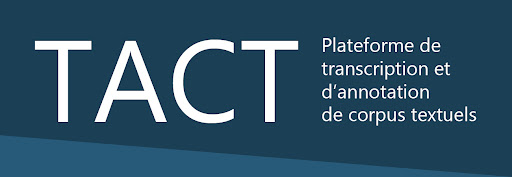
\includegraphics[width=4cm]{images/tact-logo.png}

\includegraphics[width=4cm]{images/dicto-logo.png}

\includegraphics[width=4cm]{images/elaborate-logo.png}
\end{figure}
\end{frame}

\begin{frame}[plain]
\frametitle{Pistes de travail et de r\'eflexion}
\framesubtitle{S\'election d'outils utiles}
\textbf{Manipuler et visualiser des jeux de donn\'ees}
\begin{figure}[!]

\includegraphics[width=3cm]{images/dataiku-logo.png}

\includegraphics[width=2cm]{images/openrefine-logo.png}

\includegraphics[width=3cm]{images/gephi-logo.png}

\includegraphics[width=2cm]{images/palladiologo.png}
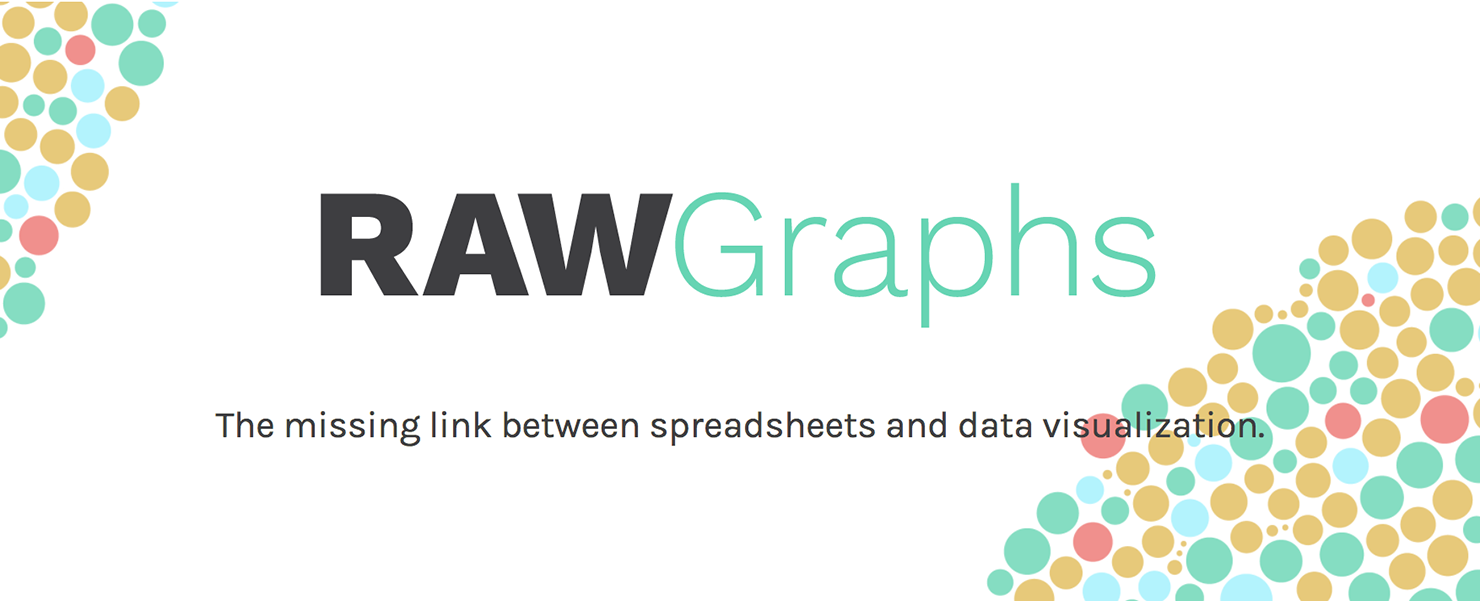
\includegraphics[width=3cm]{images/rawgraphs-logo.png}

\includegraphics[width=2cm]{images/tropy-logo.png}

\includegraphics[width=3cm]{images/voyanttools-logo.png}

\includegraphics[width=2cm]{images/tableau-logo.png}

\includegraphics[width=3cm]{images/elasticsearch-logo.png}

\includegraphics[width=2cm]{images/kibana-logo.png}
\end{figure}
\end{frame}

\begin{frame}[plain]
\frametitle{Pistes de travail et de r\'eflexion}
\framesubtitle{S\'election d'outils utiles}
\textbf{Biblioth\`eque num\'erique}
\begin{figure}[!]
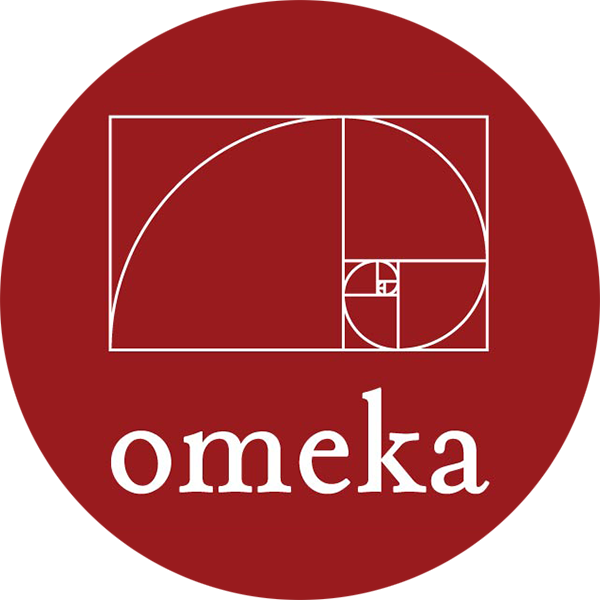
\includegraphics[width=2cm]{images/omeka-logo.png} \\
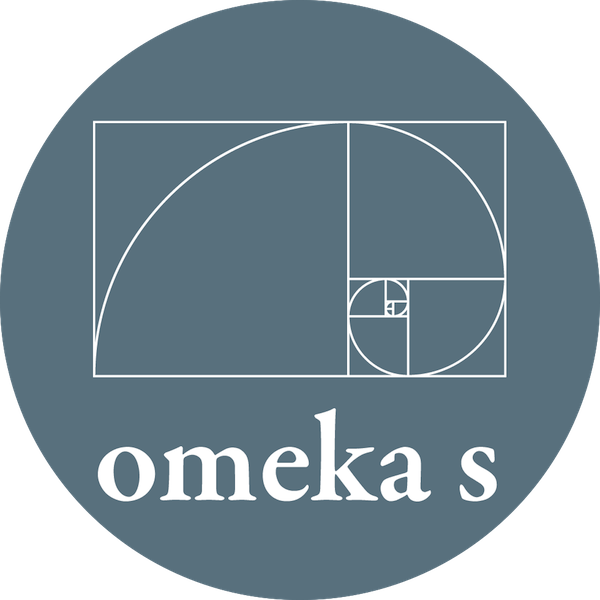
\includegraphics[width=2cm]{images/omeka-s-logo.png}\\

\includegraphics[width=2cm]{images/nakala-logo.png}\\
Nakala-Press
\end{figure}
\end{frame}

\begin{frame}[plain]
\frametitle{Pistes de travail et de r\'eflexion}
\framesubtitle{S\'election d'outils utiles}
\textbf{Cr\'eer un r\'ecit num\'erique}
\begin{figure}[!]

\includegraphics[width=3cm]{images/arcgis-storymaps-logo.png}

\includegraphics[width=3cm]{images/storymap-logo.png}

\includegraphics[width=3cm]{images/scene-logo.png}

\includegraphics[width=3cm]{images/visualeyes-logo.png}

\includegraphics[width=3cm]{images/neatline-plugin-logo.png}
\end{figure}
\end{frame}

\begin{frame}[plain]
\frametitle{Pistes de travail et de r\'eflexion}
\framesubtitle{S\'election d'outils utiles}
\textbf{Parcours d'exposition virtuelle}
\begin{figure}[!]

\includegraphics[width=2cm]{images/guidigo-logo.png}
\end{figure}
\textbf{Carte interactive}
\begin{figure}[!]

\includegraphics[width=2cm]{images/leaflet-logo.png}
\end{figure}
\begin{beamerboxesrounded}{Penser au standard \href{https://iiif.io/}{IIIF} pour les images}
\textit{International Image Interoperability Framework}, standard interop\'erable de plus en plus utilis\'e dans les applications et par les institutions culturelles, proposant des visionneuses et des API.
\end{beamerboxesrounded}
\end{frame}

\begin{frame}[plain]
\frametitle{Pistes de travail et de r\'eflexion}
\framesubtitle{Valorisation du projet : carnet Hypoth\`eses}
\begin{figure}[!]

\includegraphics[width=2cm]{images/hypotheses_logo.png}
\end{figure}
R\'edaction \`a plusieurs mains d'un article de synth\`ese ou s\'erie organis\'ee d'articles (un billet court par membre du projet).\\
\newline
Ces articles permettront de pr\'esenter :
\begin{itemize}
    \item Le choix du sujet, l'approche scientifique et la probl\'ematique
    \item La m\'ethodologie adopt\'ee (\'etapes du projet), le choix des outils num\'eriques et les limites \'eventuelles
    \item Les modalit\'es de valorisation du projet, les canaux de communication
\end{itemize}
\end{frame}

\begin{frame}[plain]
\frametitle{Ressources et Bibliographie}
\begin{itemize}
    \item GALLAND (Bruno), \textit{Les archives.}, Presses Universitaires de France, \og Que sais-je ?\fg{}, 2016, 128 pages. ISBN : 9782130748496. DOI : 10.3917/puf.galla.2016.01. \url{https://www.cairn.info/les-archives--9782130748496.htm}.
    \item Rapports annuels des archives de France : \url{https://francearchives.fr/article/37979}. 
    \item MARIN (Anne-Catherine). \og Archivistes, tous m\'ediateurs ? Petites r\'eflexions sur les pratiques professionnelles.\fg{}, \textit{La Gazette des archives}, \no247, 2017-3,pp. 145-152; doi : https://doi.org/10.3406/gazar.2017.5560.
    \item GALLAND (Bruno), NOUGARET (Christine), \textit{Les instruments de recherche dans les archives}, Paris, la Documentation fran\c caise, Direction des archives de France, 1999.
    \item BOUY\'E (\'Edouard), \textit{L'archiviste dans la cit\'e. Un ver luisant}, \'Editions Universitaires de Dijon, Collection Essais, Dijon, 2017, 105 p.
\end{itemize}
\end{frame}


\end{document}
